\documentclass[11pt]{article}
\usepackage[a4paper,margin=2.4cm]{geometry}
\usepackage{booktabs,graphicx,amsmath,hyperref,xcolor}
\hypersetup{colorlinks,linkcolor=blue!50!black,citecolor=blue!50!black,urlcolor=blue!50!black}
\usepackage[numbers,sort&compress]{natbib}

\title{Does an Explanation Stability Score Notice Data Drift?\\
\large A Reproduction and Stress Test on Three Tabular Datasets}
\author{Mithil Nagabathula\\University of East London\\\texttt{mithilnishu2000@gmail.com}}
\date{October 2026}

\begin{document}
\maketitle

\begin{abstract}
Explanation Stability Scores combine several checks on SHAP and LIME explanations into one number and gate what explanations a
production system may show. We reproduce one such score from an MSc dissertation \cite{nagabathula2026ess}
(\(\text{ESS}=0.4G+0.4L+0.2F\): global rank stability, local perturbation stability and SHAP--LIME agreement, gated at 0.75)
and stress-test it on a recruitment dataset, Adult income and German credit.
The reproduction holds (ESS \(=0.881\) on the original data), but four findings qualify it.
(1) As specified, \(G\) compares a batch's feature ranking with itself and is exactly 1 at baseline, so 40\% of the score carries no
information until a reference is fixed.
(2) Across 225 drifted batches with graded covariate shift, missingness and prior shift, the 0.75 gate never fired, even when balanced
accuracy fell by 0.33; the lowest ESS observed was 0.763. Its components moved in opposite directions: under covariate shift \(L\) rose as
\(G\) fell.
(3) ESS did fall when the \emph{model} was made unreliable with label noise or overfitting (to 0.684 and 0.715 in the worst case on two
datasets), which suggests it measures model and explanation quality rather than data drift.
(4) A calibrated variant with a held-out reference and a bootstrap threshold detected 56--95\% of harmful batches but had false alarms,
and a simple population stability index rule detected 78--95\%.
We conclude that an explanation stability score is a useful check on a model, not a drift monitor, and should sit beside input drift
statistics rather than replace them. Code and results are released.
\end{abstract}

\section{Introduction}
Regulation increasingly expects automated decisions to come with explanations \cite{euaiact2024}. Post-hoc explainers such as SHAP
\cite{lundberg2017unified,lundberg2020trees} and LIME \cite{ribeiro2016lime} are the usual tools, but their outputs can be unstable
\cite{alvarezmelis2018robustness,ghorbani2019fragile,yeh2019infidelity}, manipulable \cite{slack2020fooling} and mutually inconsistent
\cite{krishna2022disagreement}. A natural engineering response is to measure explanation stability continuously and withhold or
caveat explanations when it drops. The MSc dissertation we study \cite{nagabathula2026ess} does this inside an MLOps pipeline
\cite{kreuzberger2023mlops,sculley2015debt}: an Explanation Stability Score (ESS) gates whether a recruitment model shows full
explanations (\(\geq 0.75\)), limited explanations with a warning (\(\geq 0.60\)) or a disclaimer only.

A gate is only useful if it fires when it should. This paper asks whether ESS responds to the conditions that make explanations
untrustworthy in production: shifts in the input distribution \cite{quinonero2009shift,rabanser2019failing}, missing data, changes
in class balance, and an unreliable model. The author of this paper also wrote the dissertation; the purpose here is to test that work
critically and report what holds and what does not. Contributions:
\begin{itemize}
  \item a faithful, open reimplementation of ESS and a reproduction of the original result;
  \item a dose-response study over three datasets, three drift types and five intensities, with five seeds each;
  \item a positive control showing what ESS \emph{does} respond to;
  \item a calibrated variant and a comparison with the population stability index (PSI), the standard input-drift statistic.
\end{itemize}

\section{The score}
For a model \(f\), a batch \(X\) of \(d\) features and SHAP values \(\phi\):
\begin{description}
  \item[Global rank stability \(G\).] Rank features by mean \(|\phi|\) over \(X\). With \(r_X(j)\) the rank of feature \(j\) and
    \(r_{\text{ref}}(j)\) its rank in a reference, \(G=1-\frac{1}{d}\sum_j |r_X(j)-r_{\text{ref}}(j)|/(d-1)\).
  \item[Local stability \(L\).] For sampled rows \(x\), add Gaussian noise of 5\% of each numeric feature's standard deviation to get
    \(x'\); \(L=\text{mean}\,\max\bigl(0,1-\|\phi(x)-\phi(x')\|_1/\|\phi(x)\|_1\bigr)\).
  \item[Fidelity \(F\).] For sampled rows, the overlap of the top-5 features by \(|\phi|\) and by LIME weight, divided by 5.
\end{description}
\(\text{ESS}=0.4G+0.4L+0.2F\). In the dissertation's implementation the reference for \(G\) is the batch itself, so \(G=1\) whenever
the score is computed on a single batch. In our drift experiments the reference is the undrifted monitoring batch, which is how a
deployed monitor would have to use it. SHAP values come from CatBoost's exact TreeSHAP \cite{prokhorenkova2018catboost}.

\section{Experimental setup}
\paragraph{Data.} \emph{Recruitment}: 8{,}995 candidate offers, 14 features, 81\% joined \cite{hrdataset}; gender is excluded from the
features as in the dissertation. \emph{Adult}: a 20{,}000-row sample of the census income data \cite{kohavi1996adult}, 11 features,
race and sex excluded. \emph{German credit}: 1{,}000 applicants, 19 features, the combined sex/marital-status field excluded
\cite{hofmann1994german}.
\paragraph{Model.} CatBoost with class weighting, 500 iterations, depth 6, \(\ell_2=3\), learning rate 0.05, as in the dissertation.
\paragraph{Protocol.} For each dataset and seed (5 seeds), we split 70/30, train on the 70\%, and split the 30\% into a reference
window and a monitoring window of up to 500 rows each. ESS uses 80 rows for \(L\) and 40 for \(F\) (LIME with 2{,}000 samples).
\paragraph{Drift.} On the monitoring window we apply: \emph{covariate shift} of the five most important numeric features by
\(\{0.25, 0.5, 1, 1.5, 2\}\) standard deviations (with 30\% jitter); \emph{missingness} at rates \(\{0.1,\dots,0.8\}\) on the five most
important features (imputed as in training); and \emph{prior shift}, resampling to a positive-class share of
\(\{0.1, 0.3, 0.5, 0.9, 0.97\}\). This gives 15 drifted batches and one clean batch per seed, 240 batches in total. For each we record
ESS and its parts, mean PSI across features, and the change in balanced accuracy and AUC.

\section{Results}
\subsection{Reproduction}
On the original recruitment split, ESS was 0.881 (\(G=1\), \(L=0.883\), \(F=0.636\)), passing the full-explanation gate as reported.
Table~\ref{tab:cv} gives cross-validated performance. CatBoost had lower accuracy than a random forest but higher balanced accuracy,
the metric that matters with an 81/19 class split.

\begin{table}[t]
\centering
\caption{Predictive performance on the recruitment data, 25 runs (5 seeds $\times$ 5 folds), mean $\pm$ 95\% CI. Both models use class weighting.}
\label{tab:cv}
\small
\setlength{\tabcolsep}{4pt}
\begin{tabular}{lrrrr}
\toprule
Model & Accuracy & Balanced acc. & Macro F1 & Not-joined F1 \\
\midrule
CatBoost & 0.723 $\pm$ 0.004 & 0.688 $\pm$ 0.005 & 0.637 $\pm$ 0.004 & 0.460 $\pm$ 0.006 \\
Random Forest & 0.793 $\pm$ 0.003 & 0.640 $\pm$ 0.004 & 0.646 $\pm$ 0.004 & 0.417 $\pm$ 0.007 \\
\bottomrule
\end{tabular}
\end{table}


\paragraph{\(G\) is constant at baseline.} Because the reference is the batch itself, \(G=1\) contributes a fixed 0.4 to every
single-batch score. The informative range of ESS is therefore \([0.4, 1]\), and the 0.75 gate requires only
\(0.4L+0.2F\geq 0.35\), which holds for any model whose local stability exceeds 0.875 regardless of fidelity.

\subsection{Estimator variance}
With the dissertation's sample sizes, ESS on an unchanged batch varied with the sampling seed by a standard deviation of 0.004--0.008
(Table~\ref{tab:variance}), dominated by the LIME-based \(F\). With 20 rows for each component the standard deviation rose to 0.009--0.020
and the range of ten repetitions reached 0.058 on the recruitment data, comparable to the effect of moderate drift below.

\begin{table}[t]
\centering
\caption{Sampling variability of ESS on an unchanged batch: 10 repetitions with different sampling seeds for each local ($n_L$) and LIME ($n_F$) sample size.}
\label{tab:variance}
\small
\setlength{\tabcolsep}{4pt}
\begin{tabular}{llrrrrr}
\toprule
Dataset & $n_L$ / $n_F$ & ESS mean & ESS SD & L SD & F SD & Range \\
\midrule
Recruitment & 20 / 20 & 0.873 & 0.0200 & 0.0266 & 0.0544 & 0.058 \\
Recruitment & 80 / 40 & 0.874 & 0.0075 & 0.0126 & 0.0271 & 0.028 \\
Recruitment & 200 / 100 & 0.870 & 0.0054 & 0.0111 & 0.0159 & 0.017 \\
Adult & 20 / 20 & 0.913 & 0.0089 & 0.0132 & 0.0309 & 0.031 \\
Adult & 80 / 40 & 0.918 & 0.0037 & 0.0085 & 0.0169 & 0.011 \\
Adult & 200 / 100 & 0.917 & 0.0033 & 0.0063 & 0.0112 & 0.010 \\
German credit & 20 / 20 & 0.907 & 0.0119 & 0.0136 & 0.0387 & 0.039 \\
German credit & 80 / 40 & 0.907 & 0.0055 & 0.0082 & 0.0268 & 0.017 \\
German credit & 200 / 100 & 0.906 & 0.0024 & 0.0044 & 0.0112 & 0.008 \\
\bottomrule
\end{tabular}
\end{table}


\subsection{Dose-response under drift}
Figure~\ref{fig:dose} shows ESS, its components and the change in balanced accuracy under each drift type. Table~\ref{tab:extremes}
gives the strongest level of each.

\begin{figure}[t]
  \centering
  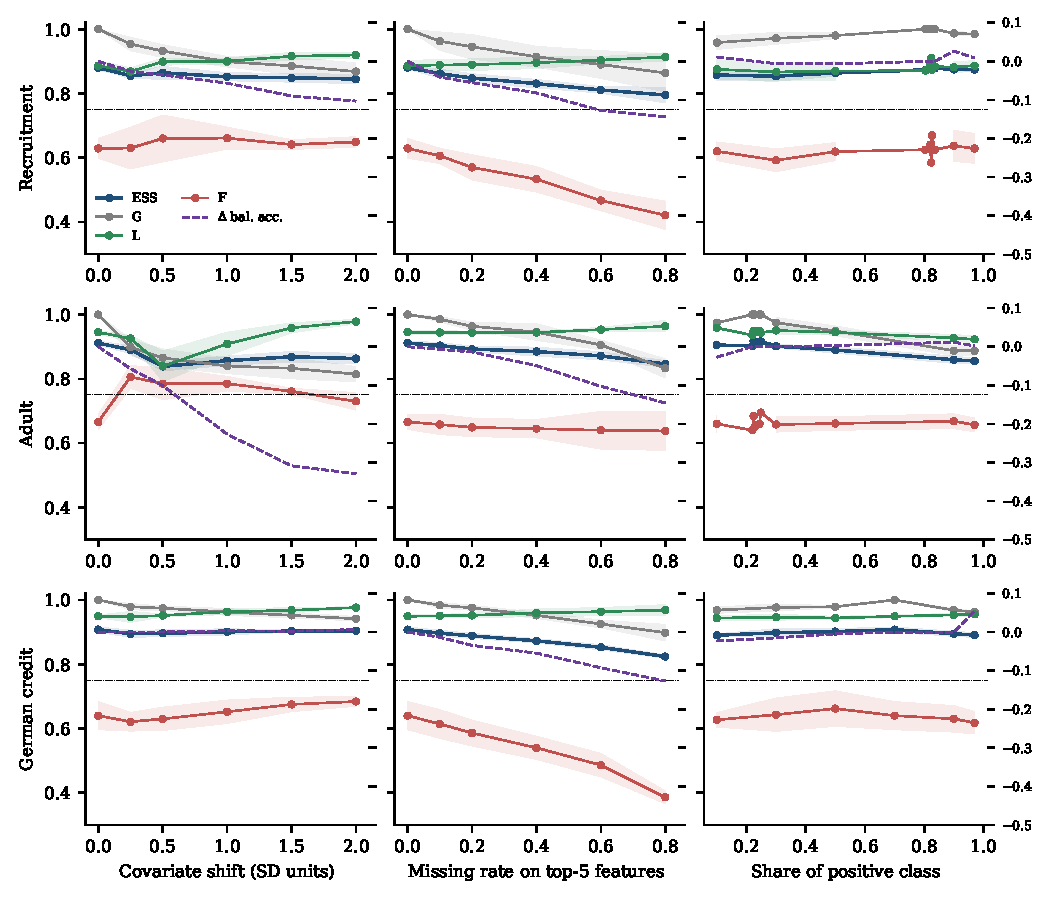
\includegraphics[width=\linewidth]{figures/dose_response.pdf}
  \caption{ESS (thick), \(G\), \(L\), \(F\) (mean \(\pm\) SD over 5 seeds, left axis) and change in balanced accuracy (dashed, right axis)
  as drift intensity increases. The dotted line is the 0.75 gate.}
  \label{fig:dose}
\end{figure}

\begin{table}[t]
\centering
\caption{ESS and its components at baseline and at the strongest level of each drift type (mean of 5 seeds). PSI is the mean population stability index across features.}
\label{tab:extremes}
\small
\setlength{\tabcolsep}{4pt}
\begin{tabular}{llrrrrrr}
\toprule
Dataset & Condition & ESS & G & L & F & PSI & $\Delta$bal.acc. \\
\midrule
Recruitment & No drift & 0.880 & 1.000 & 0.886 & 0.629 & 0.00 & -- \\
 & Covariate +2 SD & 0.845 & 0.868 & 0.920 & 0.649 & 3.15 & -0.103 \\
 & 80\% missing & 0.795 & 0.864 & 0.914 & 0.421 & 5.33 & -0.144 \\
 & Prior 97\% positive & 0.874 & 0.985 & 0.886 & 0.629 & 0.02 & +0.009 \\
Adult & No drift & 0.911 & 1.000 & 0.945 & 0.666 & 0.00 & -- \\
 & Covariate +2 SD & 0.863 & 0.815 & 0.978 & 0.730 & 1.25 & -0.330 \\
 & 80\% missing & 0.846 & 0.833 & 0.964 & 0.638 & 4.80 & -0.146 \\
 & Prior 97\% positive & 0.855 & 0.887 & 0.923 & 0.657 & 0.51 & +0.002 \\
German credit & No drift & 0.908 & 1.000 & 0.949 & 0.640 & 0.00 & -- \\
 & Covariate +2 SD & 0.904 & 0.942 & 0.976 & 0.684 & 3.45 & +0.007 \\
 & 80\% missing & 0.824 & 0.898 & 0.968 & 0.386 & 3.55 & -0.127 \\
 & Prior 97\% positive & 0.891 & 0.963 & 0.955 & 0.618 & 0.04 & +0.055 \\
\bottomrule
\end{tabular}
\end{table}


\paragraph{The gate never fired.} Across all 225 drifted batches, no ESS fell below 0.75 (Table~\ref{tab:corr}). The lowest values were
0.763 (recruitment, 80\% missing), 0.818 (German credit) and 0.825 (Adult). The largest accuracy loss, a 0.33 drop in balanced accuracy
on Adult under a 2 SD covariate shift, left ESS at 0.863.

\paragraph{Components cancel.} Under covariate shift, \(G\) fell as expected, but \(L\) \emph{rose}: on Adult from 0.945 to 0.978.
Shifting features pushes rows into flat regions of the tree ensemble, where small perturbations change SHAP values less. The
weighted sum hides the movement of \(G\). Under missingness on the recruitment and German credit data, \(F\) fell most (from 0.63 to
0.42 and from 0.64 to 0.39), probably because SHAP attributes importance to imputed values that LIME's perturbations do not reproduce.
Prior shift changed ESS by at most 0.06, and on the recruitment data by less than its own sampling noise.

\paragraph{Correlation with harm.} ESS was positively correlated with the change in balanced accuracy (Spearman \(\rho\) 0.41--0.64), so
it moves in the right direction, but too little to cross a fixed threshold. PSI correlated more strongly with harm on two of three
datasets (0.87 and 0.57) and weakly on German credit (0.15), where shifting integer-coded features produces large PSI even when
accuracy barely changes.

\begin{table}[t]
\centering
\caption{Does ESS track harm? Spearman correlation between each signal and the change in balanced accuracy over all drifted batches (75 per dataset), the share of drifted batches the dissertation's 0.75 gate would have restricted, and the lowest ESS observed.}
\label{tab:corr}
\small
\setlength{\tabcolsep}{4pt}
\begin{tabular}{lrrrr}
\toprule
Dataset & $\rho$(ESS, $\Delta$bal.acc.) & $\rho$(PSI, $-\Delta$bal.acc.) & Batches gated below 0.75 & Min.~ESS \\
\midrule
Recruitment & 0.64 & 0.87 & 0\% & 0.763 \\
Adult & 0.41 & 0.57 & 0\% & 0.825 \\
German credit & 0.44 & 0.15 & 0\% & 0.818 \\
\bottomrule
\end{tabular}
\end{table}


\subsection{Positive control}
If ESS is insensitive to drift, does it respond to anything? Table~\ref{tab:control} trains deliberately worse models: with 20\% or 40\%
of training labels flipped, and with an overfit configuration (depth 10, almost no regularisation, 1{,}500 iterations), evaluated on the
same clean audit batch. ESS fell as the model degraded in 11 of 12 degraded configurations, driven by both \(L\) and \(F\). The
combination of overfitting and 40\% label noise took it to 0.684 on recruitment and 0.715 on Adult, the only conditions in this study
that crossed the 0.75 gate; on German credit it reached 0.852, and overfitting alone left ESS unchanged (0.909 against 0.910).
\(G\) between two training runs stayed between 0.90 and 0.96 throughout and did not separate good models from bad ones. ESS is
therefore a signal about the \emph{model}: whether its attributions are smooth and whether two explainers agree about it.

\begin{table}[t]
\centering
\caption{Positive control: models made less reliable by label noise or overfitting, evaluated on the same clean audit batch (mean of 3 seeds). G (retrain) compares global rankings between two training runs of the same configuration.}
\label{tab:control}
\small
\setlength{\tabcolsep}{4pt}
\begin{tabular}{llrrrrr}
\toprule
Dataset & Model & ESS & L & F & G (retrain) & Bal. acc. \\
\midrule
Recruitment & regularised (default) & 0.879 & 0.875 & 0.645 & 0.949 & 0.693 \\
 & label noise 20\% & 0.834 & 0.809 & 0.552 & 0.952 & 0.670 \\
 & label noise 40\% & 0.819 & 0.819 & 0.457 & 0.916 & 0.598 \\
 & overfit (depth 10, l2 0.01, 1500 it) & 0.825 & 0.774 & 0.580 & 0.927 & 0.573 \\
 & overfit + label noise 40\% & 0.684 & 0.510 & 0.398 & 0.956 & 0.555 \\
Adult & regularised (default) & 0.919 & 0.955 & 0.685 & 0.921 & 0.835 \\
 & label noise 20\% & 0.901 & 0.927 & 0.650 & 0.927 & 0.818 \\
 & label noise 40\% & 0.874 & 0.911 & 0.550 & 0.927 & 0.779 \\
 & overfit (depth 10, l2 0.01, 1500 it) & 0.870 & 0.882 & 0.585 & 0.939 & 0.777 \\
 & overfit + label noise 40\% & 0.715 & 0.554 & 0.467 & 0.958 & 0.608 \\
German credit & regularised (default) & 0.910 & 0.952 & 0.647 & 0.949 & 0.692 \\
 & label noise 20\% & 0.894 & 0.928 & 0.615 & 0.928 & 0.658 \\
 & label noise 40\% & 0.861 & 0.919 & 0.467 & 0.897 & 0.556 \\
 & overfit (depth 10, l2 0.01, 1500 it) & 0.909 & 0.952 & 0.640 & 0.920 & 0.649 \\
 & overfit + label noise 40\% & 0.852 & 0.901 & 0.458 & 0.904 & 0.553 \\
\bottomrule
\end{tabular}
\end{table}


\subsection{A calibrated variant}
Two changes address the problems above: measure \(G\) against a held-out reference window rather than the batch itself, and set the
threshold from a bootstrap null distribution of no-drift batches rather than at a fixed 0.75. We call this ESS\(^\ast\) and alarm when it
falls below the 5th percentile of 30 bootstrap batches. Under the null, \(G\) averaged 0.976--0.991, and the 5th-percentile thresholds were
0.856 (recruitment), 0.906 (Adult) and 0.889 (German credit), all far above 0.75.

Table~\ref{tab:calibrated} compares detection of \emph{harmful} drift, defined as a fall of at least two points in balanced accuracy.
ESS\(^\ast\) detected 65\%, 95\% and 56\% of harmful batches where the original gate detected none. However, it raised alarms on 40\% and
20\% of clean batches on Adult and German credit, because the null was built from one seed's model and applied to models from other
seeds. A PSI rule of thumb (mean PSI \(>0.1\)) detected 78--95\% of harmful batches.

\begin{table}[t]
\centering
\caption{Detection of harmful drift (balanced accuracy down by at least 2 points) by the original fixed gate, the calibrated ESS$^{\ast}$ (held-out reference, bootstrap 5th-percentile threshold) and a PSI rule of thumb. False alarms: share of clean batches flagged by ESS$^{\ast}$. Harmful: number of harmful batches.}
\label{tab:calibrated}
\small
\setlength{\tabcolsep}{4pt}
\begin{tabular}{lrrrrrr}
\toprule
Dataset & Threshold & False alarms & ESS$^{\ast}$ & Gate 0.75 & PSI$>$0.1 & Harmful \\
\midrule
Recruitment & 0.856 & 0\% & 65\% & 0\% & 92\% & 48 \\
Adult & 0.906 & 40\% & 95\% & 0\% & 95\% & 44 \\
German credit & 0.889 & 20\% & 56\% & 0\% & 78\% & 36 \\
\bottomrule
\end{tabular}
\end{table}


\section{Discussion}
\paragraph{What ESS is good for.} The positive control suggests a clear role: as a pre-deployment and retraining check that a model's
explanations are smooth and corroborated. A model trained on noisy labels or overfit produced noticeably lower ESS on clean data.

\paragraph{What it is not good for.} As a production drift gate, ESS with a fixed threshold did not fire under any drift we applied,
including drift that cut balanced accuracy by a third. Explanation shift can be a sensitive drift signal \cite{mougan2022explanationshift},
but a weighted sum of stability components dilutes it: a self-referenced \(G\) is constant, \(L\) can rise under shift, and the 0.75
threshold sits far below the null distribution.

\paragraph{Recommendations.} (1) Compute \(G\) against a fixed reference window, or use a rank-similarity measure such as rank-biased
overlap \cite{webber2010rbo}. (2) Calibrate thresholds per model from a bootstrap null and report the false-alarm rate. (3) Monitor the
components separately, since their movements cancel. (4) Pair any explanation score with input drift statistics such as PSI.

\paragraph{Limitations.} Drift was synthetic and applied to the most important features, which is a favourable case for detection.
Three tabular datasets and one model family were studied. The bootstrap null used a single seed's model, which inflated false alarms.
The recruitment data is a public dataset of uncertain provenance. Finally, the dissertation and this paper share an author; the code is
released so that others can check both.

\section{Conclusion}
The Explanation Stability Score reproduced as reported and responded to unreliable models, but it did not notice data drift that
substantially harmed accuracy. Explanation scores should be used to vet models, calibrated against a held-out reference if used for
monitoring, and paired with conventional drift statistics.

\paragraph{Reproducibility.} Code and result files will be released at
\newline\url{https://github.com/mithil2k2000-tech/ess-drift-study}.

\paragraph{Use of AI tools.} An AI assistant (Claude, Anthropic) helped write experiment code and draft text. The author designed the
study questions, reviewed the code and results, and takes responsibility for the content.

\bibliographystyle{plainnat}
\bibliography{refs}
\end{document}
